\chapter{Traceability}
Traceability is important in every project, this project is no exception. To ensure traceability, a traceability matrix has been created. In the matrix, all the Stakeholder Needs, User Stories, Acceptance Criteria and Test IDs are listed. This ensures traceability throughout the project life-cycle.  \bigskip

%In Scrum we ally write the user stories on a little piece of paper or a "Post-it"-note. Therefor, we have chosen to represent all the user stories with "User Story Cards". All User Stories are listed later in this document.  \\
This section will describe how the Traceability Matrix is structured and what it includes. A detailed list of the activities or tasks executed throughout the project can be found in Appendix \textbf{\ref{app:tasks}}.

\section{Customer Requirements}
This project is mainly a research project and the customer has provided few initial requirements. The initial requirements given are listed below Tab. \ref{tab:custreq}.\bigskip


\begin{table}[h]
    \centering
    \begin{tabular}{|m{2cm} p{11cm} p{2cm}|}
    \hline
\rowcolor{cadetgrey}\textbf{Origin: } & \textbf{Requirement: } & \textbf{ID: } \\
                        FFI & Build a small quadcopter ($<2,5 kg$) with fixed pitch propellers & REQ001 \\ 
\rowcolor{gainsboro}    FFI & Build a small quadcopter ($<2,5 kg$) with variable pitch propellers & REQ002\\
                        FFI & Investigate if variable pitch can provide more stable flight and landing in challenging conditions & REQ003  \\ 
\rowcolor{gainsboro}    FFI & Investigate if variable pitch can improve response time of a quadcopter & REQ004\\
                        FFI & Compare the fixed pitch quadcopter with the variable pitch quadcopter & REQ005  \\
\hline

    \end{tabular}
    \caption{Customer Requirements}
    \label{tab:custreq}
\end{table}

\clearpage

\section{Stakeholder Needs}
Defining and retrieving stakeholder needs is a crucial activity, as this is where you create an understanding of what the customer wants or needs. In combination with the Traceability Matrix, it is possible to trace both User Stories and tests back to its origin. The Need section Tab. \ref{tab:stakeneeds} of the Traceability Matrix contains all the stakeholder needs, concerns and their unique need ID. 

\begin{table}[h]
    \centering
    \begin{tabular}{|m{2cm} p{1.5cm} p{9cm} p{2cm}|}
    \hline
\rowcolor{cadetgrey}\textbf{Stakeholder: } & \textbf{Origin: } & \textbf{Need: } & \textbf{Need ID: } \\
                        HSN & VAPIQ & Documentation & N001 \\ 
\rowcolor{gainsboro}    KIC & VAPIQ & The quadcopter must be able to be tested in Qualisys & N002\\
                        KIC & VAPIQ & Control the quadcopter with radio controller or external computer & N015  \\ 
\rowcolor{gainsboro}    VAPIQ & VAPIQ & Emergency switch & N018 \\
                        FFI & FFI & Build a small quadcopter ($<2,5 kg$) with fixed pitch & N008 \\ 
\rowcolor{gainsboro}    FFI & FFI & Build a small quadcopter ($<2,5 kg$) with variable pitch & N009\\
                        FFI & FFI & Investigate if variable pitch can give more stable flight and landing in challenging conditions & N022  \\ 
\rowcolor{gainsboro}    FFI & FFI & Investigate if variable pitch can improve response time & N005\\
                        FFI & FFI & Compare the fixed pitch quadcopter with the variable pitch quadcopter & N006  \\
\hline

    \end{tabular}
    \caption{Stakeholder Needs}
    \label{tab:stakeneeds}
\end{table}
\clearpage



%%%% Backlog Matrix
\section{Backlog Matrix}
The Product Backlog is represented in a Backlog Matrix displayed in Fig. \ref{fig:backlog} where all User Stories are assigned their own unique ID called "BL ID". The Backlog Matrix links all the User Stories with its corresponding Acceptance Criterion and Need ID. The unique ID makes it possible to trace everything back to the customer needs. Every story is linked to an \textbf{Epic}. An Epic is a User Story that is too big to be done in one Sprint.

\begin{table}[h]
\begin{center}
\caption{List of Epics}
\begin{tabular}{l|l}
     \rowcolor{cadetgrey} \textbf{Epic Name:}      & \textbf{JIRA ID:} \\
                        Mechanical Design                       & VPQ-1 \\  
\rowcolor{gainsboro}    Flight Controller - Software            & VPQ-2 \\  
                        Electro-Mechanical Design               & VPQ-3 \\  
\rowcolor{gainsboro}    Flight Controller - Control System      & VPQ-4 \\  
                        Communication                           & VPQ-5 \\  
\rowcolor{gainsboro}    Comparison                              & VPQ-6 \\  
                        Documentation                           & VPQ-7 \\  
\rowcolor{gainsboro}    Qualisys                                & VPQ-8 \\ 
                           
\end{tabular}
\end{center}
\end{table}
\bigskip
Below an extraction of the Backlog Matrix will follow.
\begin{figure}[h]
    \centering
        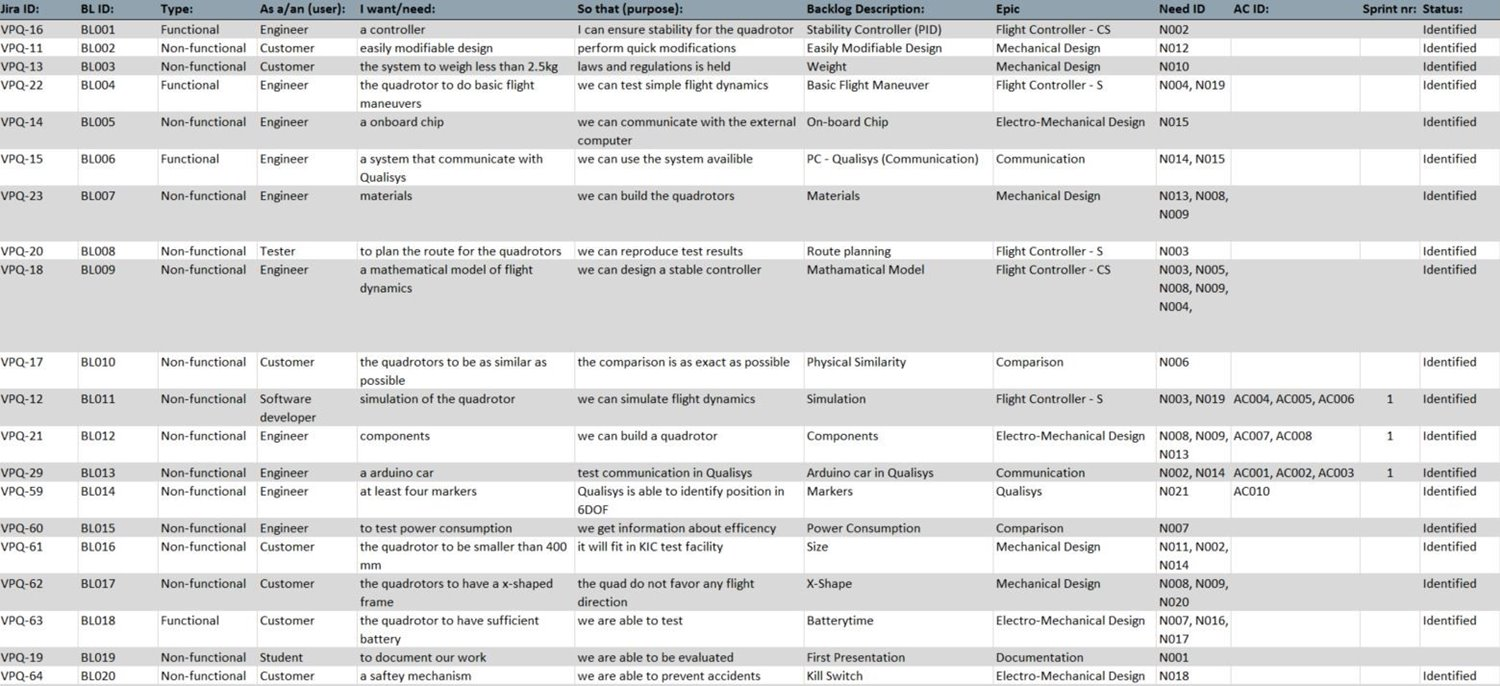
\includegraphics[width = 1\textwidth]{VAPIQ-PICTURES/BacklogMatrix}
    \caption{Extraction of the Backlog Matrix}
    \label{fig:backlog}
\end{figure}

\newpage

\section{Acceptance Criteria Matrix}
In the Acceptance Criteria section of the Traceability Matrix, Fig. \ref{fig:acm}, every Acceptance Criteria is listed with the corresponding Backlog ID. Every Acceptance Criteria gets a unique ID named AC ID with the syntax ACXXX. 
\begin{figure}[h]
    \centering
        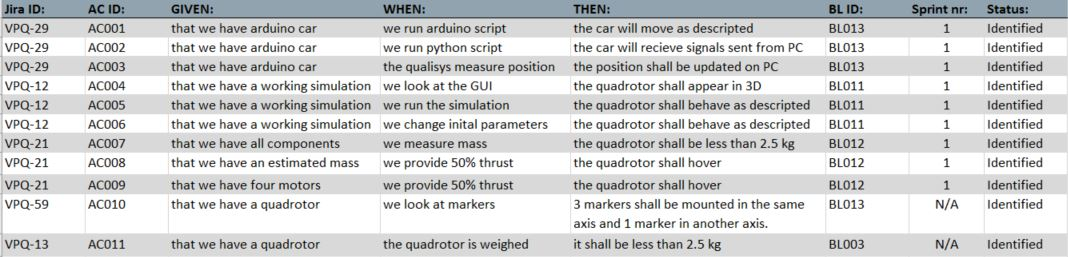
\includegraphics[width = 1\textwidth]{VAPIQ-PICTURES/AC}
    \caption{Extraction of Acceptance Criteria}
    \label{fig:acm}
\end{figure}

\newpage

\section{User Story Cards}
All Backlog Items are represented with "User Story Cards". These cards are supposed to represent the more traditional "User Story Card" often written on paper. This project utilizes User Stories as guidelines and design choices more than requirements because of the few initial requirement provided by the customer. \bigskip

This is the template for the User Story cards 

\krav{}{}{}{}{}{}{}


\textbf{BL ID} is our Backlog ID for the backlog item, this is created in the Traceability Matrix \\ \\
\textbf{Need ID} is the unique ID of the customer- or stakeholder need that the User Story are derived from. The needs can be found in the "Need" section of the Traceability Matrix \\ \\
\textbf{JIRA ID} is the automatic ID the user story gets when created in JIRA. As mentioned, all of the tasks and stories are numbered with a JIRA ID starting with VPQ (Variable Pitch Quadcopter). This ID is unique and only used in JIRA. This assures traceability between the manual Backlog and the JIRA Backlog. \\ \\
\textbf{AC ID} is the ID of the Acceptance Criterion created for the important user stories. One user story may have multiple Acceptance Criteria.  \\
\textbf{Test ID} is the ID for the test linked to the user story. \\ \\
\textbf{Sprint} is the number of the Sprint where the User Story is treated. \\ \\
\textbf{User Story} includes the User Story statement. \\
\\
